\part{Class}

\chapter{Introduction}




\section{Overview}

最简单地来说,类就是定义了一个新的类型和一个新的作用域。


\subsection{Data Structure}


类(class)是一种面向对象计算机编程语言的构造,描述了所创建的对象共同的属性和方法,用户可以使用C++中的类来定义自己的数据结构。

\subsection{Class Type}


事实上,C++设计的主要焦点就是使用类和操作符重载等来实现用户定义的类类型(class type)的行为与内置类型的一致性。例如,C++中的istream和ostream等库类型都是定义为类的,严格来说它们都不是语言本身的一部分。


类有接口和结构,而且可以将实现和接口分离。



\begin{compactitem}
\item \textsl{接口描述了如何通过方法与类及其实例互操作;}
\item \textsl{结构描述了一个实例中数据如何划分为多个属性。}
\end{compactitem}

类类型通常被称为抽象数据类型,其数据(即状态)和作用于状态的操作将被视为一个单元,因此抽象数据类型构成了面向对象编程和泛型编程的基础。



\subsection{Class Member}


类是创建对象的蓝图,其更严格的定义是由某种特定的元数据所组成的内聚的包。


类定义了数据成员和函数成员,其中:

\begin{compactitem}
\item 数据成员用于存储与类类型的对象相关联的状态,应该仅在类的私有部分定义数据成员;
\item 函数成员负责执行赋予数据意义的操作。
\end{compactitem}

类可以没有成员,也可以定义多个成员,成员可以是数据、函数或类型别名等,所有成员必须在类的内部声明。


另外,类提供了一种特殊的成员函数——转换函数来定义类类型对象之间的隐式转换,从而使编译器可以对对象实现与内置类型一致的转换。



除了定义数据和函数成员之外,类还可以定义自己的局部类型名字(或类型别名),最后以分号\footnote{按照C语言的传统,在类的定义之后接一个对象定义列表,因此类定义必须以分号结束。}结束类的定义。

\begin{lstlisting}[language=C++]
class Screen{
public:
	// interface member functions
	typedef std::string::size_type index;
private:
	std::string contents;
	index cursor;
	index height, width;
};
\end{lstlisting}

重载的成员函数和普通函数应用相同的规则:两个重载成员的形参数量和类型不能完全相同,调用非成员重载函数所用到的函数匹配过程也应用于重载成员函数的调用。

\begin{compactitem}
\item 成员函数可以被重载,但是只能重载所在类的其他成员函数。
\item 成员函数与普通的非成员函数以及在其他类中声明的函数不相关,也不能重载它们。
\end{compactitem}

\subsection{Instance}

用户在定义类实际上就是定义了一个类型,然后就可以和使用内置类型一样定义指定类型的对象。


\begin{compactitem}
\item 在类型定义阶段,编译器不进行存储分配;
\item 在对象定义阶段,编译器就会为对象分配存储空间。
\end{compactitem}


\begin{lstlisting}[language=C++]
class Screen{
public:
	// interface member functions
	typedef std::string::size_type index;
private:
	std::string contents;
	index cursor;
	index height, width;
};

Screen item;
\end{lstlisting}


一般来说,类描述了一些对象的行为规则,而这些对象就被称为该类的实例(instance),通常只有由类定义的操作可被用于对象。


\begin{compactitem}
\item 类是与某个层的对象的最具体的类型,而且类还可以有运行时表示形式(元对象),这样就可以为操作与类相关的元数据提供运行时支持。
\item 对象代表实际的存储空间,而且每个对象具有自己的类数据成员的副本。
\end{compactitem}



用户使用类来定义自己的抽象数据类型时,数据抽象能够隐藏对象的内部表示,同时仍然允许执行对象的公有(public)操作。


大多数支持类的编程语言都支持不同形式的类继承,而且许多语言还支持提供封装性的特性(比如访问修饰符)。

类为面向对象编程的三个最重要的特性(封装性、继承性和多态性)提供了实现的手段,类背后蕴藏的基本思想就是数据抽象和封装。

\begin{compactitem}
\item 数据抽象依赖于接口和实现的分离。
\item 封装将低层次的元素组合起来形成新的、高层次的的实体。
\end{compactitem}

例如,函数就是封装的一种形式,其所执行的细节行为被封装在函数中,从而可以调用一个函数,但是不能访问其所执行的语句。

封装层次更高的类也是一个封装的实体,其代表了若干成员的聚集,大多数(设计良好的)类类型都隐藏了实现该类型的成员。

例如,标准库类型vector等同时具备数据抽象和封装的特性。数组在概念上类似于vector,但是既不是抽象的,也不是封装的,用户可以通过访问存放数组的内存来直接操作数据。

并非所有类型都必须是抽象的,具体类会暴露而非隐藏其实现细节。例如标准库中的pair类就是一个实用的、设计良好的具体类(而不是抽象类),pair类型只是将两个数据成员捆绑成单个对象。


自行车制造商一遍一遍地重用相同的蓝图来制造大量的自行车,开发人员可以使用相同的类(即相同的代码)来一遍一遍地建立对象。



\section{Abstraction}


在现实世界中,经常有属于同一个类的对象,例如某辆自行车只是世界上很多自行车中的一辆。同样地,在面向对象软件中,也有很多共享相同特征的不同的对象—矩形、雇用记录和视频剪辑等,可以利用这些对象的相同特征为它们建立一个蓝图。

对象的软件蓝图就是类,通过类可以定义所有一类对象的变量和方法的蓝图或原型。例如,可以建立一个定义包含当前档位等实例变量的自行车类,这个类也定义和提供了实例方法(变档、刹车)的实现。

\begin{compactitem}
\item 类不是它描述的对象,例如自行车的蓝图不是自行车,对象则是现实世界的电子模型或抽象概念。
\item 抽象类被定义为永远不会也不能被实例化为具体的对象。
\end{compactitem}

实际上,抽象类往往用于定义一种抽象上的概念,在类的继承关系中它往往被定义在较上层的位置。

抽象类与接口存在类似的地方,二者都偏重于对共通的方法和属性进行规约,但是抽象类往往可以规约一个共同的方法和属性时提供一个对他们的实现。

以现实世界为例,"水果"可以算作一个抽象类,"苹果"和"香蕉"则可以作为它的派生类,它们的区别在于"水果"是个概念,它不会有实例,但是"苹果"和"香蕉"则肯定会有实例。

实例变量的值由类的每个实例提供。例如,当创建自行车类以后,必须在使用之前对它进行实例化。



当创建类的实例时,就建立了这种类型的一个对象,然后系统为类定义的实例变量分配内存,这样就可以调用对象的实例方法来实现一些功能。

相同类的实例共享相同的实例方法。除了实例变量和方法,类也可以定义类变量和类方法。

操作系统在第一次在程序中遇到一个类时为这个类建立它的所有类变量的拷贝 - 这个类的所有实例共享它的类变量。


从类的实例中或者从类中都可以访问类变量和方法。类方法只能操作类变量,不必访问实例变量或实例方法。



\section{Encapsulation}

所有的面向对象编程语言都共有这些相同的概念:类、实例、消息传递、方法和继承等。


用户可以从多个角度考虑面向对象编程(尤其是对象),因此在不同的面向对象编程语言中,使用不同的术语来表示相似概念是很普遍的事情。

在面向对象设计中引入了不同的抽象层次,通过这些层次来检查程序,这样从高级抽象的角度可以将对象看作是抽象数据类型的实例。

数据抽象是一种有效的解决问题的方式,它将某些信息有意识地隐藏在程序的某个部分。例如,用户开发的一系列抽象数据类型都可以从两个方面来看待。

与Parnas原则相似,从外部来看,抽象数据类型的客户(用户)只能看到抽象行为的操作集合,作为抽象数据类型的另一接口,定义抽象的实现者通过数据变量可以来维护对象的内部状态。

例如,对于堆栈(Stack)的抽象,用户只能看到合法操作的描述—如push、pop和top。另一方面,实现者需要了解用来实现抽象的具体数据结构,这样具体的细节就被封装在更加抽象的框架中。

\begin{figure}[htbp]
\centering
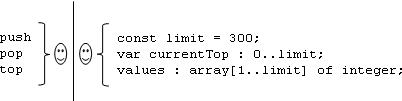
\includegraphics[scale=0.6]{stack.png}
\caption{堆栈的接口和实现}
\label{fig:stack}
\end{figure}

一般使用实例(instance)来表示类的一个具体代表或范例。相应地,使用实例变量(instance variable)来表示实例所维护的内部变量,有时也会使用数据字段(data field)或数据成员(data members)来表示这一概念。

每个实例都有它自己的实例变量集合,客户不能直接改变这些值,只有和类相关的方法才能改变它们。

对象可以简单地看作状态(state)和行为(behavior)的结合,其中状态由实例变量来描述,而行为由方法来表示。

\begin{compactitem}
\item \textsl{从对象外部来看,客户只能看到对象的行为;}
\item \textsl{从对象内部来看,方法通过修改对象的状态以及和其他对象的相互作用来提供适当的行为。}
\end{compactitem}

\chapter{Declaration}


\section{Forward Declaration}


用户在只声明一个C++类时称为前向声明(forward declaration),结果是在程序中引入了一个不完全类型(incompete type)的类类型,这样就可以用来编写相互依赖的类。

不完全类型只能以有限方式使用,不能定义该类型的对象,因此不完全类型只能用于定义指向该类型的指针及引用,或者用于声明(而不是定义)使用该类型作为形参类型或返回类型的函数。



在创建类的对象、使用引用或指针访问类的成员之前,必须完整地实现不完全类型的类类型,这样编译器才能给类的对象预定相应的存储空间。

\begin{compactitem}
\item 只有当类定义已经定义过,数据成员才能被指定为该类类型。
\item 如果类是不完全类型,数据成员只能是指向该类类型的指针或引用。
\end{compactitem}

类不能具有自身类型的数据成员,但是可以具有指向自身类型的指针或引用的数据成员。

\begin{lstlisting}[language=C++]
class LinkScreen{
	Screen window;
	LinkScreen *next;
	LinkScreen *prev;
};
\end{lstlisting}

\section{Forward Definition}

在实践中,有时需要两个或者更多的互相引用的类,这种形式称为相互递归(mutual recursion)。例如,在表示马和马车的关系时,每一匹马需要和自己的马车联系在一起,每一辆马车又需要有一匹马。

很多语言都支持相互递归,例如Java语言在生成代码之前会扫描整个文件,这样如果程序文件的前面部分引用在文件后面声明的类,就不会产生任何冲突。

其他的语言(例如C++)会从前到后地依次处理程序文件中的类和方法,因此名称在使用之前必须至少进行部分定义。


在C++语言中必须实现向前定义(forward definition),其目的只是把这个名称置于循环中,关于定义的实现会在后面完成,这样马和马车的例子可能需要进行一定的修改。

\begin{lstlisting}[language=C++]
class Horse; // forward definition

class Buggy{
	...
	Horse * myHorse;
};

class Horse{
	...
	Buggy* myBuggy;
};
\end{lstlisting}

这里,首行仅仅表明Horse是一个类的名称,定义即将在后面出现。

对于C++编译器来说,只需知道前向定义的相关信息才能允许创建指向未知类的指针。当然,在读取类定义之前,对象不能做任何事情。

要解决这种问题,需要对类定义和与其相关的方法的实现仔细地排序:首先是第一个类的定义,然后是第二个类的定义,紧接着是第一个类的方法,最后是第二个类的方法。

\chapter{Definition}

根据语言是动态类型还是静态类型,可以把语言分为静态类型和动态类型两大类。

一般来说,静态类型语言中类型和变量有关(这种绑定通常是通过声明语句来建立的),在动态类型语言中只是把变量看作名称标识,类型和值有关。

\begin{compactitem}
\item Java、C++、C\#和Pascal语言是静态类型语言;
\item Smalltalk、CLOS和Python语言是动态语言类型;
\item Objective-C语言介于这两种类型语言之间。
\end{compactitem}

在Objective-C语言中,如果变量是静态类型,则变量可以用一个固定类型来声明。另一方面,变量也可以使用对象类型id来声明。通过这种方式声明的变量可以表示任何值,因此这种变量是动态类型。

\begin{lstlisting}[language=bash]
PlayingCard aCard;	/* a statically typed veriable */
id anotherCard;		/* a dynamically typed veriable */
\end{lstlisting}

在消息传递方面,静态类型语言和动态类型语言之间存在显著的差异。

一方面,静态类型语言在编译时使用接收器的类型来检查选择器,以确定它所接收的消息。

另一方面,动态类型语言在编译时则没有办法去核实这一消息,因此在动态类型语言中如果接收器不理解消息选择器,消息就可能产生运行时错误,静态类型语言就从来不会发生这种运行时错误。

\section{Overview}

如果通过在玩纸牌游戏来对纸牌进行抽象,可以通过一系列的细化来扩展纸牌的抽象,其中的每一次细化都会加入少量的新特征。

首先,设想将一张纸牌抽象成一个容器,那么该容器包含纸牌花色和纸牌点数这两个数据值,然后用1~13这些数字来表示纸牌的点数(1代表A纸牌,11、12、13分别代表J、Q和K纸牌)。

\begin{compactitem}
\item 如果使用的编程语言支持枚举(enum),那么可以使用枚举数据类型来表示花色。
\item 如果使用的语言不支持枚举数据类型,则可以使用符号常量和从1~4的整数值来表示花色。
\end{compactitem}


枚举数据类型的优点是可以避免类型错误,因此可以保证一张纸牌的花色一定是四种指定数值之一。如果使用整数来表示花色,就无法防止程序员把无效的整数值赋给纸牌花色变量(例如100)。



下面分别是使用不同语言(C++、Java、C\#)对类的定义的示例。

\begin{lstlisting}[language=C++]
// C++
class PlayingCard {
public:
	enum Suits { Spade, Diamond, Club, Heart };
	
	Suits suit() { return suitValue; }
	int rank() { return rankValue; }
	
private:
	Suits suitValue;
	int rankValue;
};
\end{lstlisting}

\begin{compactitem}
\item 在一个给定的C++源文件中,一个类只能被定义一次。
\item 在多个源文件中定义一个类时,每个源文件中的类定义必须是完全相同的。
\end{compactitem}





\begin{lstlisting}[language=Java]
// Java 
class PlayingCard {
	public int suit() { return suitValue; }
	public int rank() { return rankValue; }
	
	private int suitValue;
	private int rankValue;
	
	public static final int Spade = 1;
	public static final int Diamond = 2;
	public static final int Club = 3;
	public static final int Heart = 4;
}
\end{lstlisting}



\begin{lstlisting}[language={[Sharp]C}]
// C#
class PlayingCard {
enum Suits { Spade, Diamond, Club, Heart };
	public Suits suit() { return suitValue; }
	public int rank() { return rankValue; }
	
	private Suits suitValue;
	private int rankValue;
}
\end{lstlisting}


\section{Visibility}



类的可视性(visibility,又叫可访问性)修饰符用于定义抽象接口和实施封装。

\begin{compactitem}
\item C++语言的访问修饰符和冒号标明整块说明语句;
\item Java和C\#的访问修饰符分别放在每一条语句之前。
\end{compactitem}


在面向对象编程语言中都提供了一种方式用来区别以下这两种情况:一种是可以被类定义的外部(outside)了解和使用的特征,另一种是只能用于类定义内部(within)的特征。其中,后者由关键词private来表示,也就是说使用访问修饰符(public、private等)可以控制类的可视性和可操作性特征。

如果类是用struct关键字定义的,则在第一个访问修饰符之前的成员都是公有的,如果类是用class关键字定义的,则这些成员都是私有的。

\begin{compactitem}
\item 类型的数据抽象视图由其public成员定义。
\item private封装了类型的实现细节。
\end{compactitem}




在C++和C\#语言中,可以定义枚举数据类型来表示纸牌花色。其中,C++语言通过将定义语句放置在类中,可以清晰地表达这两种数据类型之间的联系。

对于C++语言,在类定义之外表示花色的常量必须以类名为前缀:

\begin{lstlisting}[language=C++]
if(aCard.suit() == PlayingCard::Diamond) ...
\end{lstlisting}

对于C\#语言,以枚举类型名为前缀:


\begin{lstlisting}[language=C++]
if(aCard.suit() == Suits.Diamond) ...
\end{lstlisting}

这里,aCard是PlayingCard(纸牌)的一个实例的名称,通过调用suit方法可以检查纸牌的花色。数据字段suitValue和rankValue表示这一抽象的实例数据。每一个PlayingCard类的实例都有自己独立的数据字段,用来维护自己的花色和点数值。

注意,花色值是通过调用suit()这一方法得到的,suit()方法只是简单地返回数据字段suitValue的数值。

大多数语言遵循的惯例是将类名的首字母大写,但并不是所有的语言都这样,尤其是C++程序中更多的是全部使用小写字母来表示类名。


一般情况下,实例变量的命名不需要首字母大写,目的是为了更容易区分类型名和实例变量名。


在Java语言还没有提供枚举数据类型\footnote{从Java 5.0开始引入了枚举类型。}时,通常的做法是定义一系列的符号常量。这里,符号常量需要使用两个修饰符final和static来修饰。

\begin{compactitem}
\item 修饰符final表示这个名称所表示的值不再改变。
\item 修饰符static的意义是不管对这个类创建多少实例,static所修饰的变量实例都只有一个。
\end{compactitem}

final和static修饰符一起作用时,就定义了一个不能改变的唯一变量—也就是常量(constant)。


在使用Java来定义类时,需要注意数据字段suitValue、rankValue和常量Spade、Diamond、Club、Heart之间的区别。其中,后者是由static来修饰的,因此它们存在于任何一个类实例的外部,并且被所有的实例共享,这类似于过程式语言中的全局变量。另外,数据字段suitValue和rankValue不是静态的,因此每个类实例都会有关于这两个数据字段的副本。

Apple公司的Object Pascal语言和Borland公司的Delphi Pascal语言(在Linux平台上称为Kylix)都是基于早期简单的Pascal语言的,因此来自原始语言的很多特征都是一样的,它们都对Pascal语言以各自的方式进行了相应的扩展。

\begin{lstlisting}[language=Pascal]
/* Object Pascal */
type 
	Suits = (Heart, Club, Diamond, Spade);
	
	PlayingCard = object
		suit : Suits;
		rank : integer;
	end;

/* Delphi Pascal */
type 
	Suits = (Heart, Club, Diamond, Spade);
	
	TPlayingCard = class(TObject)
		public 
			constructor Create(r : integer; s : Suits);
			
			function suit : Suits;
			function rank : int;

		private
			suitValue : Suits;
			rankValue : integer;
	end;
\end{lstlisting}



Object Pascal和Delphi Pascal语言都支持枚举数据类型,其中:

\begin{compactitem}
\item 前者使用关键字object来声明一个新类,因此类有时被称为对象类型(object types)。
\item 后者使用关键字class来声明新类,而且要求每一个类都必须从已有的类继承而来,这里通过继承TObject来创建新类。
\end{compactitem}

在Delphi中,类的命名惯例是以大写字母T来开头,而且Delphi语言支持访问修饰符,而Apple语言却不使用访问修饰符。另外,Delphi语言需要构造函数。


Smalltalk语言实际上不使用文本来表示类,而是使用一种称为browser的交互式界面来描述。例如,下图显示了browser的屏幕快照。

\begin{figure}[htbp]
\centering
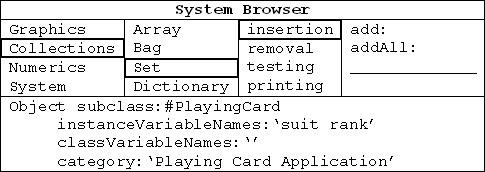
\includegraphics[scale=0.6]{smalltalk_class.jpg}
\caption{Smalltalk浏览器示意图}
\label{fig:smalltalk_class}
\end{figure}

在Browser中,用户通过将消息传递给父类Object来定义一个新类。

与Delphi Pascal语言一样,Smalltalk语言中的所有的类也必须继承于一个特定的父类。例如,上面的示意图说明了包含两个数据字段实例的PlayingCard类的创建。

下面分别是使用其他的不同语言(CLOS、Eiffel、Objective-C)对类的定义的示例。



\begin{lstlisting}[language=Lisp]
// CLOS
(defclass PlayingCard() (rank suit))
\end{lstlisting}






\begin{lstlisting}[language=Eiffel]
// Eiffel
class PlayingCard
feature 
	Spade, Diamond, Heart, Club : Integer is Unique;
	
	suit : integer;
	rank : integer;
end
\end{lstlisting}





\begin{lstlisting}[language={[Objective]C}]
enum suits { Heart, Club, Diamond, Spade };
@ interface PlayingCard : Object
{
	suits suit;
	int rank;
}
@end
\end{lstlisting}


对于类是面向对象编程最基本的概念的思想,一些语言中在其之上进行了一些改变。

Oberon语言中对于类只有比较传统的数据记录的概念。尽管如此,它还是支持消息传递以及面向对象思想中才有的对方法进行动态绑定的功能。

Oberon语言中的方法不是在记录内定义的,而是使用特殊的语法来声明方法,在参数列表中,使用一个与其他参数位置分离的参数来描述接收器。通常要求接收器是指针类型,而不是数据记录类型。

\begin{lstlisting}[language=Oberon-2]
TYPE
	PlayingCard = POINTER TO PlayingCardDesc;
		
	PlayingCardDesc = RECORD
		suit : INTEGER
		rank : INTEGER
		faceUp : BOOLEAN
	END
PROCEDUER (aCard : PlayingCard) setFaceUp (b : BOOLEAN)
BEGIN
	aCard.faceUp = b;
END
\end{lstlisting}


记录PlayingCardDesc包括数据字段,可以通过过程setFaceUp来修改数据字段,而过程setFaceUp作为接收器,必须得到关于纸牌的指针。

\section{Context}


成员函数有一个附加的隐含实参(this指针\footnote{C++类的成员函数具有一个附加的隐含形参,即指向类对象的一个this指针,与调用成员函数的对象绑定在一起。})来将函数绑定到调用函数的对象。

\begin{compactitem}
\item 成员函数不能定义this形参,只能由编译器隐含地定义。
\item 成员函数的函数体可以显式使用this指针。
\end{compactitem}

如果对类成员的引用没有限定,编译器将会把对隐含指针的引用处理成通过this指针的引用。

在成员函数内部显式引用this通常是不必要的,只有一种情况下(即需要将一个对象作为整体引用而不是引用对象的一个成员)才必须显式引用this指针,最常见的就是函数需要返回对调用该函数的对象的引用。

某些类的操作可能需要返回引用时就会使用this指针并返回*this。例如,在下面的Screen类中的单个表达式中调用move和set操作时,每个操作必须返回一个引用。

\begin{lstlisting}[language=C++]
class Screen{
public:
	// interface member functions
	Screen& move(index r, index c);
	Screen& set(char);
	Screen& set(index, index, char);
	// other members before
};
\end{lstlisting}

这里,move和set函数的返回类型时Screen\&,说明它们返回对自身类类型的对象的引用,而且每个函数都返回调用自己的对象,这里就可以使用this指针来访问对象。


下面set和move实现中,每个函数都返回*this,this本身是一个指向非常量Screen的指针,因此可以通过对this指针解引用来访问this指向的对象。

\begin{lstlisting}[language=Oberon-2]
Screen& Screen::set(char c)
{
	contents[cursor] = c;
	return *this;
}
Screen& Screen::move(index r, index c)
{
	index row = r * width; // row location
	cursor = row + c;
	return *this;
}
\end{lstlisting}

用户不能从const成员函数返回指向类对象的普通引用,而且const成员函数只能返回*this作为一个const引用。

\begin{compactitem}
\item 在普通的非const成员函数中,this的类型是一个指向类类型的const指针,可以改变this所指向的值,但是不能改变this所保存的地址。
\item 在const成员函数中,this的类型是一个指向const类类型对象的const指针,既不能改变this所指向的对象,也不能改变this所保存的地址。
\end{compactitem}

例如,为了给Screen类增加一个display操作来在给定的ostream上打印contents,必须定义两个display操作,而且const对象只能使用const成员,非const对象可以使用任一成员。

\begin{compactitem}
\item 基于成员函数是否为const来重载成员函数;
\item 基于指针形参是否指向const来重载成员函数。
\end{compactitem}



\begin{lstlisting}[language=C++]
class Screen{
public:
	// interface member functions
	// display overloaded on whether the object is const or not
	Screen& display(std::ostream &os)
	{
		do_display(os);
		return *this;
	}
	Screen& display(std::ostream &os) const
	{
		do_display(os);
		return *this;
	}
private:
	// single function to do the work of displaying a Screen,
	// will be called by the display operations
	void do_display(std::ostream &os) const
	{
		os << contents;
	}
	// as before
};
\end{lstlisting}

\section{Scope}

每个类都定义了自己的新作用域和唯一的类型,在类的定义体内声明类成员,将成员名引入类的作用域,而且两个不同的类具有两个不同的作用域。

即使两个类具有完全相同的成员列表,它们也是不同的类型,每个类的成员不同于任何其他类(或任何其他作用域)的成员。


\begin{lstlisting}[language=C++]
class First{
public:
	int memi;
	double memd;
};
class Second{
public:
	int memi;
	double memd;
};

Frist obj1;
Second obj2;
obj2 = obj1; // error, obj1 and obj2 have different types
\end{lstlisting}

在类作用域之外,成员只能通过对象或指针分别使用成员访问操作符(.或->)进行访问,而且成员访问操作符的左边的操作数分别是一个类对象或指向类对象的指针,跟在操作符后面的成员名字必须在相关联的类的作用域中声明。




\begin{lstlisting}[language=C++]
Class obj;
Class *ptr = &obj;
ptr->member;
obj.member;
ptr->memfcn();
obj.memfcn();
\end{lstlisting}

除了使用成员访问操作符来访问成员之外,也可以直接通过类使用作用域操作符(::)来访问,一般的数据或函数成员必须通过对象来访问。

在类的定义体之外出现的成员定义必须指明成员所在的类,而且形参表和成员函数体都出现在函数名之后,但是它们仍然属于类的作用域,因此可以不用限定而引用其他成员。

\begin{lstlisting}[language=C++]
double Sales_item::avg_price() const
{
	if(units_sold)
		return revenue/units_sold;
	else
		return 0;
}
\end{lstlisting}

与形参类型相比,返回类型出现在成员名字前面,并且需要遵循如下规定:

\begin{compactitem}
\item 如果函数在类定义体之外定义,则用于返回类型的名字在类作用域之外;
\item 如果返回类型使用由类定义的类型,则必须使用完全限定名。
\end{compactitem}

\begin{lstlisting}[language=C++]
class Screen{
public:
	typedef std::string::size_type index;
	index get_cursor() const;
};
inline Screen::index Screen::get_cursor() const
{
	return cursor;
}
\end{lstlisting}

在类的作用域中进行名字查找\footnote{名字查找(name lookup)是寻找与给定的名字使用相匹配的声明的过程。}时,首先在使用该名字的块中查找名字的声明,如果找不到则在包围的作用域中查找,在找不到任何声明的情况下将报错。

实际上,C++类定义在两个阶段中处理,在第一阶段中编译成员声明,在所有成员出现之后才编译它们的定义本身,因此C++要求所有名字必须在使用之前声明,

类作用域中使用的名字并非

\begin{lstlisting}[language=C++]

\end{lstlisting}




\begin{lstlisting}[language=C++]

\end{lstlisting}



\begin{lstlisting}[language=C++]

\end{lstlisting}




\begin{lstlisting}[language=C++]

\end{lstlisting}



\begin{lstlisting}[language=C++]

\end{lstlisting}



\subsection{C++}

C++中的类可以控制在初始化、复制、赋值和销毁对象时发生的操作,用户使用类可以为要解决的问题定义定制的数据类型,从而方便开发易于理解的应用程序。

一般情况下,C++类定义在以.h结尾的头文件中,要使用类的任何程序都必须使用\#include命令包含头文件,从而保证在每个使用类的文件中都以同样的方式来定义类。

\begin{compactitem}
\item 每个类定义一种类型,类型名与类名相同;
\item 内置类型和类类型都可以定义变量。
\end{compactitem}

使用头文件保护符(header guard)可以保证即使头文件在同一个文件中被包含多次,类定义也只会出现一次。

\begin{lstlisting}[language=C++]
#ifndef SALESITEM_H
#define SALESITEM_H

#include <iostream>
#include <string>
class Sales_item{
...
};
#endif
\end{lstlisting}


按照惯例,头文件存储类类型的定义,而且头文件名和类名一样,头文件可以以.h、.H、.hpp或.hxx等后缀名。

在C++类内部,声明成员函数是必需的,但是定义成员函数则是可选的。

\begin{compactitem}
\item 在类内部定义的函数默认为inline。
\item 在类外部定义的成员函数必需必须指明所在类的作用域。
\end{compactitem}



如果将关键字const放在形参表之后,就可以将成员函数声明为常量,const成员不能改变其所操作的对象的数据成员。

\begin{quote}
\texttt{const必须同时出现在声明和定义中,否则就会出现一个编译时错误。}
\end{quote}

在类内部定义的成员函数(例如不接受实参的get函数)将自动作为inline处理,也就是说,当编译器在它们被调用时将试图在同一行内扩展它们,也可以显式地将成员函数声明为inline。

\begin{lstlisting}[language=C++]
class Screen{
public:
	typedef std::string::size_type index;
	char get() const { return contents[cursor]; }
	inline char get(index  ht, index wd) const;
	index get_cursor() const;
	...
};

char Screen::get(index r, index c) const
{
	index row = r * width;
	return contents[row+c];
}
inline Screen::index Screen::get_cursor() const
{
	return cursor;
}
\end{lstlisting}

用户在声明和定义处指定inline都是合法地,而且在类的外部定义inline可以使类容易阅读。

\begin{compactitem}
\item 在类定义体内部的声明中指定成员为inline;
\item 在类定义体外部的定义中指定成员为inline。
\end{compactitem}

inline成员函数的定义必须在调用该函数的每个源文件中时可见的,通常应该将不在类定义体内定义的inline成员函数的定义放在有类定义的同一头文件中。

用户在定义了类类型之后,可以按照以下两种等价的方式使用。

\begin{compactitem}
\item 将类的名字直接用作类型名;
\item 指定关键字class或struct,后跟类的名字。
\end{compactitem}

\begin{lstlisting}[language=C++]
Screen screen;
class Screen screen;
\end{lstlisting}



\subsection{Java}



\subsection{C\#}


\subsection{Python}


Python语言的格式是逐级缩进的,它不包含用来指示类、函数和语句嵌套的开始和结束符。


\begin{lstlisting}[language=C++]
class PlayingCard:
	"A playing card class"
	def __init__(self, s, r)
		self.suit = s
		self.rank = r
\end{lstlisting}


\subsection{PHP}




\begin{lstlisting}[language=PHP]
class PlayingCard {
	enum Suits { Spade, Diamond, Club, Heart };
	private Suits $suitValue;
	private int $rankValue;
	
	public Suits suit(){
		return $suitValue;
	}
	public int rank(){
		return $rankValue;
	}
}
\end{lstlisting}



\subsection{Ruby}



\begin{lstlisting}[language=Ruby]
class PlayingCard {
	Suits {Spade, Diamond, Club, Heart}
	attr_reader :suitValue, :rankValue;
	def initialize(suitValue, rankValue)
		@suitValue, @rankValue = suitValue, rankValue
	end
	def <=>(card)
		suitValue <=> card.suitValue
		rankValue <=> card.rankValue
	end
	def to_s
		"#{suitValue} (#{rankValue})"
	end
end
}
\end{lstlisting}







\section{Nested Class}

Java和C++中都允许在一个类中定义另外一个类,在Java中称其为内部类,在C++中则称为嵌套类。


尽管上述这两个概念有相似的表现,但它们之间也有很大的语义区别。

在Java中,内部类被链接到与其相关的外部类的一个具体实例上(内部类就创建在这个外部类实例中),并且允许存取这一对象的数据字段和方法。

在C++中,嵌套类只是一种简单的命名手段,它限制了和内部类相关的特征的可视性,除此之外,两者再没有其他关系。

为了说明嵌套类的作用,假设想要用Java语言来写一个双向链表的抽象,可能决定把Link类放在List抽象中。



\begin{lstlisting}[language=Java]
// Java List Class
class List{
	private Link firstElement = null;
	public void push_front(Object val){
		if(firstElement == null)
			firstElement = new Link(val, null, null);
		else
			firstElement.addBefore(val);
	}
	... // other methods omitted 
	private class Link{ // inner class definition
		public Object value;
		public Link forwardLink;
		public Link backwardLink;
		public Link(Object v, Link f, Link b){
			value = v;
			forwardLink = f;
			backwardLink = b;
		}
		public void addBefore(Object val){
			Link newLink = new Link(val, this, backwardLink);
			if(backwardLink == null){
				firstElement = newLink;
			}else{
				backwardLink.forwardLink = newLink;
				backwardLink = newLink;
			}
		}
		... // other methods omitted
	}
}
\end{lstlisting}

注意,方法addBefore()引用数据字段firstElement的目的是为了处理这种一种特殊情况,就是将一个元素插入到链表的头部。

如果将上述代码直接转换成C++语言来表示,就会产生如下的结果。


\begin{lstlisting}[language=C++]
// C++ List Class
class List {
private:
	class Link; // forward definition
	Link *firstElement;
	
	class Link { // nested class definition
	public:
		int value;
		Link *forwardLink;
		Link *backwardLink;
		
		Link(int v, Link *f, Link *b){
			value = v;
			forwardLink = f;
			backwardLink = b;
		}
		
		void addBefore(int val){
			Link *newLink = new Link(val,  this, backwardLink);
			if(backwardLink == 0){
				firstElement = newLink; // Error!
			}else{
				backwardLink->forwardLink = newLink;
				backwardLink = newLink;
			}
		}
		... // other methods omitted
	};
	
public:
	void push_front(int val){
		if(firstElement == 0){
			firstElement = newLink (val, 0, 0);
		}else{
			firstElement->addBefore(val);
		}
	}
	... // other methods omitted
};
\end{lstlisting}


在上面示例代码中,正是由于Link类的向前引用,才使得在定义Link类之前,就可以声明关于Link类的指针firstElement。

C++语言也使用数值0来表示空元素,而不是通过伪常量null来表示空元素。对Link的使用是通过指针,而不是数值,因此必须进行指针的存取操作。但是,对代码行的注释信息显示了相应的出错代码。

内部类的范围实际上没有嵌套于外部类,因此Link类禁止存取变量firstElement。为了存取List对象,可以通过一个变量来显式进行。对于这一实例,最合理的解决方案就是使用伪变量this,把List方法作为一个参数传递给Link的内部方法addBefore(另一种替代的方式,就是使每个Link对象都包含一个关于与其相关的List的引用,但是这样做有些过于浪费内存)。



\begin{lstlisting}[language=C++]
class List {
	Link *firstElement;
	
	class Link{
		void addBefore(int val, List *theList){
			...
			if(backwardLink == 0){
				theList->firstElement = newLink;
			}
			...
		}
	};
public:
	void push_front(int val){
		...
		// pass self as argument
		firstElement->addBefore(val, this);
	}
	... // other methods omitted
};
\end{lstlisting}

当嵌套类的方法定义于类主体之外时,方法的名称就需要通过多级限定来表示。例如,下面这个示例展示了方法addBefore通过这种形式进行编码的情形。



\begin{lstlisting}[language=C++]
void List::Link::addBefore(int val, List *theList){
	Link *newLink = new Link(val, this, backwardLink);
	if(backwardLink == 0){
		theList->firstElement = newLink;
	}else{
		backwardLink->forwardLink = newLink;
		backwardLink->newLink;
	}
}
\end{lstlisting}

在上述的示例中,函数的名称表明这是一个名称为addBefore的方法,并且这个方法是Link类的一部分,同样,Link类又被定义为List类的一部分。

\section{Meta Class}


为了理解Smalltalk和其他语言中的元类(metaclass)的概念,首先要提到一种和对象无关,但却和类相关的方法。也就是说,假设我们创建了纸牌对象,则不会在对象自身中发现和纸牌相关的方法,但是却可以在类PlayingCard中找到这一方法。例如,在下面的示例中,在类PlayingCard中找到与纸牌相关的方法。

\begin{figure}[htbp]
\centering
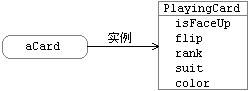
\includegraphics[scale=0.6]{playingcard_meta.png}
\label{fig:playingcard_meta}
\end{figure}


在Smalltalk语言中,类就是对象。类自身就是可以对特定消息作出响应,比如用来创建对象的消息new。例如,在下面所示的示意图显示了类自身对特定消息作出响应。


\begin{figure}[htbp]
\centering
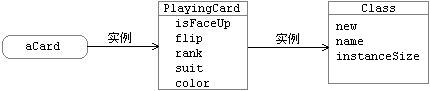
\includegraphics[scale=0.6]{smalltalk_meta.png}
\label{fig:smalltalk_meta}
\end{figure}

假设有这样一种情况,我们想要创建一个可以用在构造函数中的方法,即我们需要一种方法——假设为rank: suit:,它可以传递给具体的类对象——假设为PlayingCard,当执行方法时,将创建一个新的实例并确保这个实例被正确地初始化。在这种情况下,这个方法应该放在什么地方呢?它不可能是PlayingCard的成员方法,因为它是类实例所执行的方法,而在创建类的时候我们还没有实例。它也不是Class的成员方法,因为Class的成员方法对所有的类都是通用的,而这个初始化方法只是针对这一个类有效。

解决方案是创建一个新的“隐藏”类,称为元类(metaclass),名字为PlayingCard的对象实际上不是Class的实例,而是MetaPlayingCard的实例,而MetaPlayingCard则继承于Class。与初始化相关的特定行为可以置于这个元类中。


\begin{figure}[htbp]
\centering
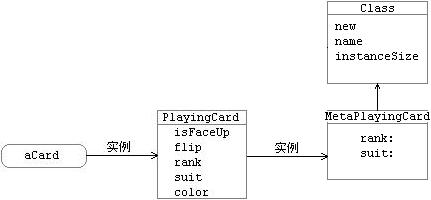
\includegraphics[scale=0.6]{acard_meta.png}
\label{fig:acard_meta}
\end{figure}

类MetaPlayingCard中的行为,只能被对象PlayingCard所理解,而不能被其他对象所理解。对象PlayingCard是类MetaPlayingCard的唯一实例。

Smalltalk浏览器通常对用户隐藏元对象,我们把这样的方法称为类方法(class method),它们看起来就像与类相关联一样,但是在浏览器背后,类方法只是和元类相关联的普通方法。


\begin{lstlisting}[language=C++]

\end{lstlisting}





\begin{lstlisting}[language=C++]

\end{lstlisting}




\chapter{Method}



\section{Overview}


关于纸牌抽象的进一步改进,包括以下几个方面:

\begin{compactitem}
\item 增加一种方法,可以返回纸牌的颜色(红色还是黑色);
\item 增加一个数据字段,来表示纸牌是面朝上还是面朝下,并且增加检测这一数据字段值状态的方法和翻转纸牌的方法。
\end{compactitem}


使用C\#定义的用来表明这些变化的一个典型的类如下所示:

\begin{lstlisting}[language={[Sharp]C}]
class PlayingCard{
	// constructor, initialize new playing card
	public PlayingCard(Suits is, int ir){
		suit = is;
		rank = ir;
		faceup = true;
	}
	
	// operations on a playing card
	public Boolean isFaceUp(){
		return faceup;
	}
	public Suits suit(){
		return suitValue;
	}
	public int rank(){
		return rankValue;
	}
	public void setFaceUp(Boolean up){
		faceUp = up;
	}
	public void flip(){
		setFaceUp(!faceUp);
	}
	public Color color(){
		if((suit() == Suits.Diamond) || (suit() == Suits.Heart))
			return Colors.Red;
		return Color.Black;
	}
	
	// private data values
	private Suits suitValue;
	private int rankValue;
	private Boolean faceUp;
}
\end{lstlisting}



其中,需要注意的特征就是增加了第二个枚举数据类型来表示颜色,并且又增加了以private来修饰的第3个数据字段来表示纸牌面朝上状态。

将数据字段声明为private意味着禁止从类定义的外部来存取该数据字段,从而确保了修改该数据字段的唯一方式就是使用与这个类相联系的方法。

大多数的面向对象编程方式指南都会建议,数据字段永远不应声明成public,而应该是private或者protected。

构造函数是一种特殊的方法,它们有着和类相同的名称,并且用于在对象中初始化数据字段。

\subsection{getter}


类必须对外提供一种存取数据字段的方法,通过定义于类中的方法来存取数据字段是一种好的面向对象编程方式。

仅仅返回数据字段值的方法称为存取器(accessor),有时也称为获取器(getter)。这里,getter方法的一个实例是isFaceUp,它返回数据字段faceUp的值。另外一个例子是方法rank,它返回数据字段rankValue的值。


为什么对这个简单的行为使用一个方法,而不是直接存取数据字段来实现呢?

一个原因就是方法可以使数据字段是只读的(read-only)。函数只能被调用,而数据字段既可以读又可以写,因此通过private数据字段和public存取器的结合,我们可以确保纸牌的点数一旦创建,就不会被改变。


这里所使用的对方法的命名是一种典型的命名约定。以is开头命名一个返回布尔值的方法是很好的做法,它清楚地表示了当方法返回真值时所代表的含义。按照这一约定,可以更容易理解条件语言中使用的方法,如下所示:

\begin{lstlisting}[language={[Sharp]C}]
if(aCard.isFaceUp())...
\end{lstlisting}


这里,aCard是PlayingCard类的一个实例。很多编程方式指南建议存取器方法以get这个词开始,这样可以清晰地表明,该方法最主要的目的仅仅是获取数据字段的值。这一约定也使得使用这种方法的语句更容易理解,如下所示:



\begin{lstlisting}[language={[Sharp]C}]
int cardRank = aCard.getRank();
\end{lstlisting}

然而,这一约定并不适用于任何情况,尤其是当为这些方法使用更简单的名称rank和suit时。

\subsection{setter}


主要目的仅仅是设置字段值的方法称为可变器(mutator)或者设置器(setter),设置器的命名通常以单词set开始。例如,方法setFaceUp就是设置器的一个实例,它用来设置存取器faceUp的值。


\begin{lstlisting}[language={[Sharp]C}]
class PlayingCard{
	...
	void setFaceUp(Boolean up){
		faceUp = up;
	}
	...
}
\end{lstlisting}

flip方法既不是获取器也不是设置器,因为它既没有获取数据字段值,也没有设置数据字段值。它只是一个简单的方法。方法color从技术上来说也不是获取器,因为它没有获得关于这个类的数据字段值。尽管如此,但由于它返回了对象的一个属性,所以一些编程指南建议,getColor是一个更好的命名。


Smalltalk语言不支持访问修饰符。

缺省情况下,Smalltalk语言中的所有数据字段都是private(即只能在类定义内部进行存取)。为了存取数据字段,必须提供相应的存取器方法:


\begin{lstlisting}[language=bash]
rank 
	" return the face value of a card "
	'$\uparrow$' rank
\end{lstlisting}



Smalltalk语言并没有广泛地遵循以单词get开始的命名约定。通常情况下,Smalltalk语言中存取器方法与它们返回的数据字段同名。

获取器和设置器函数(或者称为存取器和可变器),通过它们可以对数据字段进行存取,这样使用方法而不是直接存取数据字段,用户可以更加灵活地控制数据的修改方式以及确定数据所处的位置。


\section{Declaration}


一般说来,并不指定在类定义中方法的声明次序,不过次序对代码的可读性有很大的影响。

\begin{compactitem}
\item 在类定义中,首先列出一些主要的特征,一些次要的特征列在后面。
\item 构造函数是对象定义的一个最重要的方面,因此应该位于类定义的顶部。
\item 对方法的声明应该通过分组来表示,这样可以迅速便捷地找到对应于给定消息选择器的方法。分组的原则可以按照字母顺序排列,或者按照方法的职能进行分组。
\item 私有数据类型只是对于类的开发者才重要,它们应该列在类定义中靠后的位置。
\end{compactitem}


在面向对象编程中,消息总是传递给接收器。然而,在大多数面向对象语言中,接收器并不出现在方法的参数列表中,而是隐藏于方法的定义之中,也就是说用来响应消息的方法在方法体内部存取消息接收器。

只有当必须从方法体内部去存取接收器的数值时,才会使用伪变量(pseudo-variable)。伪变量和通常的变量很相似,只是它不需要声明,也不能被更改(因此这里也许使用伪常量更加合适,只是伪常量从未出现在任何语言的定义中)。

\begin{compactitem}
\item 在Java和C++语言中,由伪变量表示的接收器命名为this;
\item 在Eiffel语言中称为Current;
\item 在Smalltalk、Objective-C、Object Pascal等语言中称为self。
\end{compactitem}

伪变量在使用时就好像是作为类的一个实例。例如,方法color可以用Pascal语言编写成如下结果:

\begin{lstlisting}[language=Pascal]
function PlayingCard.color : colors;
begin
	if(self.suit = Heart) or (self.suit = Diamond) then
		color := Red
	else
		color := Black;
end
\end{lstlisting}

在很多编程语言中,对接收器伪变量的使用都可以忽略。如果在没有引用接收器的条件下,访问一个数据字段或者调用一个方法,那么这意味着接收器伪变量将作为消息的主体。

例如,PlayingCard中的flip方法就体现了这一点,flip方法就是通过调用setFaceUp方法来实现它的功能的:



\begin{lstlisting}[language=Java]
class PlayingCard{
	...
	public void flip(){
		setFaceUp(!faceUp);
	}
}
\end{lstlisting}

使用伪变量可以将这一方法重新编写,从而使接收器显示出来,如下所示:



\begin{lstlisting}[language=Java]
class PlayingCard{
	...
	public void flip(){
		this.setFaceUp(!this.faceUp)
	}
}
\end{lstlisting}

当某一方法想要把自身当作一个参数传递给另外一个函数时,就必须使用变量来解决问题。



\begin{lstlisting}[language=Java]
class QuitButton extends Button implements ActionListener{
	public QuitButton(){
		...
		//install ourselves as a listener for button events
		addActionListener(this);
	}
	...
}
\end{lstlisting}

对于构造函数,使用this和构造函数的参数初始化数据成员。通过显式地使用this,可以区分用作函数参数和数据成员的两个同名变量。


\begin{lstlisting}[language=Java]
class PlayingCard{
	public PlayingCard(int suit,int rank){
		this.rank = rank; //this.rank is the data member
		this.suit = suit; //rank is the argument value
		this.faceUp = true;
	}
	...
	private int suit;
	private int rank;
	private boolean faceUp;
}
\end{lstlisting}

Python、CLOS和Oberon等语言则不遵循上述原则,接收器必须在方法体中显式地声明。例如,在Python语言中,一条消息可以包含两个参数,如下所示:




\begin{lstlisting}[language=Python]
aCard.moveTo(27,3)
\end{lstlisting}

相应的方法需要声明3个参数值:


\begin{lstlisting}[language=Python]
class PlayingCard:
	def moveTo(self, x, y):
		...
\end{lstlisting}


对于这些语言,尽管原则上第一个参数可以以任何名称来命名,但是一般都命名为self或者this,以此来表示该方法与接收器伪变量之间的关系。

在CLOS和Oberon语言中,也必须把接收器命名为方法的一个参数。


\begin{lstlisting}[language=Java]

\end{lstlisting}




\begin{lstlisting}[language=Java]

\end{lstlisting}

\section{Constant}

一些编程语言提供了一种方式来作为存取器方法的一种替代,可以指定一个数据字段是可变的或者是不可变的,从而意味着如果设定了数据字段的值,就不能再改变它,就没有必要通过方法来隐藏对数据值的存取。


下面描述了关于定义常量的不同方式。例如,在Java中是用final来声明常量的,在C++中则使用修饰符const来实现。


\begin{lstlisting}[language=C++]
// C++
class PlayingCard{
public:
	...
	const int rank; // since immutable, can allow public access to data field.
	const Suits suit;
};
\end{lstlisting}


\begin{lstlisting}[language=Java]
// Java
class PlayingCard{
	...
	public final int rank;
	public final Suits suit;
}
\end{lstlisting}


常量(或者称为不可变数据字段)直观地说明了在程序执行过程中不能改变其值的数据字段。





\section{Isolation}

Java和C\#等都是把方法的主体直接放在类定义中,而C++和Object Pascal等语言则是将这两方面分离开来。

在C++语言中可以自由选择,小规模的方法可以在类内部定义,大规模的方法可以在类外部定义。例如,一个关于纸牌抽象的C++类定义如下所示:

\begin{lstlisting}[language=C++]
// C++ 
class PlayingCard{
public:
	enum Suits { Spade, Diamond, Club, Heart };
	enum Colors { Red, Black };
	// constructor, initialize new playing card
	PlayingCard(Suits is, int ir){
		suit = is;
		rank = ir;
		faceUp = true;
	}
	// operations on a playing card
	boolean isFaceUp(){ // bool
		return faceUp;
	}
	void setFaceUp(bool up){
		faceUp = up;
	}
	void flip(){
		setFaceUp(!faceUp);
	}
	int rank(){
		return rankValue;
	}
	Suits suit(){
		return suitValue;
	}
	
	Colors color();

private: // private data values
	Suits suitValue;
	int rankValue;
	boolean faceUp; // bool
};
\end{lstlisting}

注意,这里忽略了方法color的实现主体,因为它的实现代码比在类中所定义的其他方法都要长。随后的方法定义(又称为函数成员,function member)提供了函数的主体。


\begin{lstlisting}[language=C++]
// C++
PlayingCard::Colors PlayingCard::color(){
	// return the face color of a playing card
	if((suit == Diamond) || (suit == Heart))
		return Red;
	return Black;
}
\end{lstlisting}

方法标题定义的格式和通常的C语言函数定义十分类似,只是名称已经扩展成为一个全限定(fully qualified)名,而且这种受限定的名称由类的名称和定义的方法名称组成,如同一个人是由姓和名来确定的一样(例如“Jim Green”)。

C++程序员既可以将方法作为类定义的一部分,定义成内联(in-line)方法,也可以将方法定义成程序的一个独立的部分。

一般情况下,把只有一到两个语句的方法定义成内联方法,把多于两行的复杂语句定义在类的外部。



把方法体放在类定义之外有两个原因。首先,多余一条语句的方法体会使类定义的其他特征变得模糊,因此移开代码比较长的方法体可以改善程序的可读性。只是,可读性是针对观察者的,而不是所有的用户都认为这种分离可以提高程序的可读性,因为这样做之后,用户就必须到两个不同的地方去查找方法的主体。

第二个原因涉及到语义。当方法体在一个类定义内部被声明时,C++编译器就可以直接将其作为内联方法进行扩展,而无需建立函数调用,这样内联方法比函数调用和方法体的结合形式执行起来更加快速。


在C++语言程序中,通常不会在同一个文件中同时出现类定义和较大的方法体。

\begin{compactitem}
\item 类声明一般会在接口文件(interface file)中给出(按照惯例,在UNIX系统中是扩展名为.h的文件,在Windows系统中是扩展名为.hpp的文件)。
\item 函数体位于实现文件中(按照惯例,是扩展名为.cpp或.C的文件)。
\end{compactitem}

Objective-C语言也把类定义和类实现分离开来。其中,类定义包括关于类的方法的描述,它们通过符号“+”或者“-”来指示,随后紧接着位于括号之内的返回类型,返回类型之后是方法的描述。

\begin{lstlisting}[language={[Objective]C}]
@ interface PlayingCard : Object
{
	int suit;
	int rank;
	int faceUp;
}
	
+ suit: (int) s rank: (int) i
- (int) color;
- (int) rank;
- (int) suit;
- (int) isFaceUp;
- (void) flip;
@ end
\end{lstlisting}


关于方法体的实现代码如下:



\begin{lstlisting}[language={[Objective]C}]
@ implementation PlayingCard
	
- (int) color
{
	if((suit == Diamond)||(suit == Heart))
		return Red;
	return Black;
}
- (int) rank
{
	return rank;
}
... ./* other method bodies */
@ end
\end{lstlisting}



Object Pascal和Delphi语言分离类定义和方法函数体的方式很相似,分离的这两个部分都是保存在同一个文件中。类定义描述位于以interface为标识的部分,而具体实现代码位于以implementation为标识的部分。例如,下面就是一个Delphi语言的示例。


\begin{lstlisting}[language=C++]
interface
type
	Suits = (Heart,Club,Diamond,Spade);
	Colors = (Red,Black);
	
	TPlayingCard = class (TObject)
		public
			constructor Create (r : integer; s : Suits);
			function color : Colors;
			function isFaceUp : boolean;
			procedure flip;
			function rank : integer;
			function suit : Suits;
		private
			suit : Suits;
			rank : integer;
			faceUp : boolean;
	end;	
implementation
	function TPlayingCard.color : Colors;
	begin
		case suit of
			Diamond: color := Red;	
			Heart: color := Red;
			Spade: color := Black;
			Club: color := Black;
	end

...(* other methods similarly defined *)
end;
\end{lstlisting}



在Pascal语言中的全限定名是通过在类名和方法名之间使用句点分隔而成,C++语言则是使用冒号来进行分隔。

CLOS语言在进行类定义时,可以通过使用“:accessor”关键字和位于其后的存取器函数名,自动地创建存取函数。


\begin{lstlisting}[language=Lisp]
// CLOS
(defclass PlayingCard()
	((rank :accessor getRank) (suit :accessor getSuit) ))
\end{lstlisting}

其他的方法是使用函数defmethod来定义的,而且方法的接收器以一个显式参数来命名,这一点和Java以及C++语言是不同的。





\begin{lstlisting}[language=Lisp]
// CLOS
(defmethod color((card PlayingCard))
	(cond
		((eq (getSuit card) ‘Diamond) ‘Red)
		((eq (getSuit card) ‘Heart) ‘Red)
		(t 'Black)))
\end{lstlisting}

在Python语言中,接收器也必须以显示参数命名。




\begin{lstlisting}[language=Python]
class PlayingCard:
def __init__(self, s, r):
	self.suit = s
	self.r = r
def rank(self):
	return self.rank
def color(self):
	if self.suit == 1 or self.suit == 2:
		return 1
	return 0
\end{lstlisting}


\section{Message}


\begin{compactitem}
\item 面向对象语言的静态特征包括如何创建新的数据类型、新的类和新的方法等。
\item 面向对象语言的动态特征涉及到值是如何实例化(或者被创建)的,它们又是如何初始化的,以及它们如何通过消息传递来相互联系。
\end{compactitem}

在面向对象编程思想中,创建(实例化)就是为一个新对象分配存储空间并且将这段空间与对象名称进行绑定。

实际上,初始化不但包括为对象的数据区域设置初始值(类似于对记录中的数据字段进行的初始化),还包括建立操作对象所需的初始条件这个更一般的过程。

在大多数面向对象语言中,后者对于使用对象的客户的隐藏程度是封装的一个重要的方面,这也被认为是面向对象技术优于其他编程技术的一个主要方面。

使用消息传递(message passing,或称为method lookup,方法查询)这一术语来表示请求对象执行一项特定行为的动态过程。例如,在Fred送花给Cris的示例中,非正式地描述了消息传递,并且指明了如何区分消息和通常的过程调用。

\begin{compactitem}
\item 消息总是传递给某个称为接收器的对象;
\item 响应消息所执行的行为不是固定不变的,它们根据接收器类的不同而不同。
\end{compactitem}

不同的对象可以接收相同的消息,但是却执行不同的行为,因此对于任何消息传递表达式都有3个确定的部分,它们是接收器(receiver,消息传递的目的对象)、消息选择器(message selector,表示待传递的特定的消息文本)和用于响应消息的系数(argument)。

\begin{figure}[htbp]
\centering
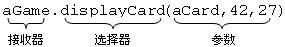
\includegraphics[scale=0.65]{message.png}
\caption{消息传递表达式}
\label{fig:message}
\end{figure}

消息传递最通常的语法是使用句点来把接收器和消息选择器分离开来,还有一些次要的变化特征。例如,在方法没有参数时,是否需要使用一对空的圆括号(在Pascal和一些其他的语言中可以省略这对圆括号)。

\begin{lstlisting}[language=C]
// C++, C#, Java, Python, Ruby
aCard.flip();
aCard.setFaceUp(true);
aGame.displayCard(aCard,45,56);
// Pascal, Delphi, Eiffel, Oberon
aCard.flip;
aCard.setFaceUp(true);
aGame.displayCard(aCard,45,56);
// Smalltalk
aCard flip.
aCard setFaceUp: true.
aGame display: aCard atLocation: 45 and: 56.
// Objective-C
[ aCard flip ].
[ aCard setFaceUp: true ].
[ aGame display: aCard atLocation: 45 and: 56 ]
// CLOS
(flip aCard)
(setFaceUp aCard true)
(displayCard aGame 45 56)
\end{lstlisting}

在Smalltalk和Object-C语言中,表示消息传递的语法有一些细微的差异,使用空格作为分隔符。一元消息(不含参数的消息)只是简单地写在接收器之后。含有参数的消息使用关键字表示法(keyword notation)。消息选择器被分成几个部分,每个参数之前都有一个部分。冒号跟在每个关键字之后。

\begin{lstlisting}[language=C++]
aGame display: aCard atLocation: 45 and: 56.
\end{lstlisting}


在Smalltalk语言中,即使是二元操作(例如加法)也被解释为将右值参数传递给左值的消息。

\begin{lstlisting}[language=C++]
z <- x + y. " message to x to add y to itself and return sum "
\end{lstlisting}

在C++语言中定义的二元操作符也表示相似的含义。

在Object-C语言中,将一条类似于Smalltalk语言的消息包含在方括号中,称为消息传递表达式。方括号只包括消息本身,而不包括其他内容。例如,不包括存放消息结果的变量。


\begin{lstlisting}[language=C++]
int cardrank = [ aCard getRank ];
\end{lstlisting}


CLOS语言中的语法遵循传统的Lisp语法。Lisp语言中的所有表达式都写成以圆括号为边界的列表。操作是列表的第一个元素,紧接着是参数。接收器是第一个参数。



\chapter{Property}



\section{Overview}

编程语言(包括面向对象语言和非面向对象语言)都包含一种称为属性的概念。在语法上,属性是以数据字段的方式来进行操作的,但是像方法一样,它也是内部操作。也就是说,属性既可以作为表达式来读取,也可以对其进行赋值。




\begin{lstlisting}[language=C++]
Writeln('rank is', aCard.rank); (* rank is property of card *)
aCard.rank = 5; (* changing the rank property *)
\end{lstlisting}

无论是读取属性值还是对属性赋值,都必须通过函数来实现,而不是仅仅由一个简单的数据值来实现。

Delphi语言中的属性是通过关键字property以及修饰符read和write来声明的,紧跟read和write关键字之后的可以是数据字段,也可以是方法名。

当某一属性用在表达式的形式中,read属性就会被会调用,而当属性作为赋值目标时,write属性就会被调用。只能读取而不能写入的属性称为只读属性。

例如,在下面的示例中,对属性的修改作为属性的纸牌点数值和花色值。







\begin{lstlisting}[language=C++]
type
	TPlayingCard = class(TObject)
		public
				
			property rank : Integer read rankValue;
			property suit : Suits read suitValue write suitValue;
		private
			rankValue : Integer;
			suitValue : Suits;
	end;
\end{lstlisting}

这里,我们把点数定义成只读属性,而将花色定义成读写属性,也可以定义一个只写属性,只是这很少用。


在C\#中,属性是通过编写一个无参数的方法来定义的,这个方法只包括一个get部分或者一个set部分,其中:

\begin{compactitem}
\item get部分必须返回一个值;
\item set部分可以使用伪变量value来设置属性。
\end{compactitem}

\begin{lstlisting}[language={[Sharp]C}]
public class PlayingCard{
	public int rank{
		get{
			return rankValue;
		}
		set{
			rankValue = value;
		}
	}
	...
	private int rankValue;
}
\end{lstlisting}

\begin{compactitem}
\item 如果只有get部分而没有提供set部分,则属性为只读属性。
\item 如果只有set部分而没有提供get部分,则属性为只写属性。
\end{compactitem}

在C\#程序中,属性通常是无参数且返回惟一值的函数。

\subsection{C++}


\begin{lstlisting}[language=C++]

\end{lstlisting}




\subsection{Java}


\begin{lstlisting}[language=C++]

\end{lstlisting}



\subsection{C\#}



\begin{lstlisting}[language=C++]

\end{lstlisting}

\section{Mutable}

如果希望类的数据成员(包括在const成员函数内)可以修改,可以将它们声明为mutable。

可变数据成员永远都不能为const,因此const成员函数可以改变mutable成员,需要使用关键字mutable来声明数据成员。

\begin{lstlisting}[language=C++]
class Screen{
public:
// interface member functions
private:
	mutable size_t access_ctr; // may change in const members
	// other data members as before
};
\end{lstlisting}







\chapter{Field}

使用被一个类的所有实例共享的公共数据字段,在解决许多问题时都非常方便。然而,对这样的对象进行的操作却为面向对象语言的设计者创建了一个奇特的矛盾。

为了理解这个问题,考虑一下当初创建类这个概念的原因——就是要减少创建相似对象的工作量。类的每一个实例都和这个类的其他实例有着完全一致的行为。现在,假设由于某种原因我们定义了一个公共数据字段,它可以被类的所有实例共享,然后考虑如何对公共数据字段进行初始化。这看起来有两种选择,但是每种选择都不能令人满意。一种选择是每个实例都执行对公共数据字段的初始化任务(字段初始化后,还会被反复地初始化),另一种选择是没有实例执行初始化任务(数据字段一直处于未初始化状态)。

为了解决这一矛盾,我们需要从类/方法/实例这个简单的实例中跳出来进行思考,因此另外一个机制就是,对象本身不必对共享数据进行初始化。

如果对象通过内存管理器自动将共享数据初始化为一个特定值(例如0),那么每一个实例都可以测试这一特定值,并且如果它们是第一个进行测试的实例,它们就会对数据进行初始化。不过,还应该有其他的更好的方法。

在C++和Java语言中,共享数据字段都是使用static修饰符来创建的。例如,在Java语言的符号常量创建中,就会使用这种办法。

一般情况下,Java语言中的静态数据字段的初始化是在加载类时,通过执行静态块(static block)来完成的。例如,假设我们想要了解一个类已经创建了多少个实例,可以通过下面的方法来实现。

\begin{lstlisting}[language=Java]
class CountingClass{
	CountingClass(){
		count = count + 1; // increment count
		...
	}
	...
	private static int count; // shared by all
	static { // static block
		count = 0;
	}
}
\end{lstlisting}

C++语言有两种不同的方法,其中由基本数据类型表示的静态数据字段(或常量)可以在类的主体中进行初始化,或者也可以在类之外对静态数据字段进行全局的初始化。



\begin{lstlisting}[language=C++]
class CountingClass{
pubilc:
	CountingClass(){
		count ++;
		...
	}

private:
	static int count;
};

// global initialization is separated from class
int CountingClass::count = 0;
\end{lstlisting}

C\#语言可以通过静态构造方法(声明为static的构造方法)来对静态数据字段进行初始化,而且构造方法不允许有任何参数。


使用关键字static就解决了以前关于初始化一个类的所有实例共享数据字段所引起的特殊矛盾。

Python语言中的类的数据字段在方法层次上命名,而实例变量在方法内部命名(一般在构造方法内部)。

\begin{lstlisting}[language=Python]
class CountingClass:
	count = 0
	def __init__(self):
		self.otherField = 3
\end{lstlisting}



\section{Anonymous Class}

在很多面向对象语言中,类本身就是一个对象。

在多数情况下,有一个特殊的类(一般称为Class),这就是类的类,而且它们具有相应的行为。例如,通常创建类的一个实例就是简单地给类对象传递一条消息。




下面是Smalltalk中的相应示例:

\begin{lstlisting}[language=C++]
aCard<-PlayingCard new. "message new given to object PlayingCard"
\end{lstlisting}

其他的一般行为包括返回类的名称、类实例大小或者类实例可识别的消息列表。

在非交互式语言中,有时很难表示程序语句和程序输出之间的关系,在实际的程序开发中要能够区分可执行语句和非执行的输出结果。例如,下面的Java代码就说明了这些应用:




\begin{lstlisting}[language=C++]
Object obj = new PlayingCard();
Class c = obj.getClass();
System.out.println("class is " + c.getName());
\end{lstlisting}

至于类是否是面向对象编程所必需的,现代软件开发技术中已经证明,不使用类而通过委托(delegation)就可以实现面向对象语言的大多数期望的特征。

不过,从委托语言的第一次提出到现在,它并没有得到完全支持,所以大多数用户更愿意使用类。


\subsection{Java}

在某些应用场景中,用户需要创建一个简单的、不多于一个实例的类,这样的对象称为单件(singleton)。


Java提供了创建这样的对象的一种机制,甚至不需要对这样的对象所涉及的类进行命名,因此这样的类称为匿名类(anonymous class)。

为了创建匿名类,需要以下几个条件:

\begin{compactenum}
\item 只能创建一个匿名类的实例;
\item 匿名类必须继承于父类或接口,并且不需要构造函数进行初始化。
\end{compactenum}

在GUI(用户界面)的环境下,经常会遇到这种情况。例如,我们在设计一个用于创建图形按钮的类ButtonAdapter时,为了提供关于按钮的行为,程序员必须建立一个继承于ButtonAdapter的新类,并且改写方法pressed。

如果只需要一个这种对象,可以通过匿名类(又叫类定义表达式,class definition expression)来完成。

在使用方法add将图形元素添加到窗口时,为了将新按钮添加到窗口中,需要以下代码:


\begin{lstlisting}[language=Java]
Window p = ...
p.add(new ButtonAdapter("Quit"){
		public void pressed(){System.exit(0);}
	}
);
\end{lstlisting}

通过查看传递给add操作符的参数,会发现参数涉及一个新值的创建,通过add操作符来实现。

但是,这个关于new的参数列表的表达式并没有以反括号结束,而是又出现了一个花括号。实际上,这是一个新类的定义。创建了一个基于ButtonAdapter的子类,并且创建了一个关于这个子类的实例。这个新类所需的所有方法都通过内联函数给出。

在这个实例中,新类改写了名为pressed的方法,最后通过反花括号结束了匿名类表达式。


\chapter{Constructor}

构造函数(construtor)是用来初始化一个新创建对象的方法,而且构造函数本身可以重载。

\begin{compactitem}
\item 构造函数用于给每个数据成员设置适当的初始值;
\item 构造函数应用初始化列表来初始化对象的数据成员。
\end{compactitem}

构造函数的初始化列表由成员名和带括号的初始值组成,跟在构造函数的形参表后面,并以冒号开头。

\begin{lstlisting}[language=C++]
// default constructor needed to initialize members of built-in type
Sales_item(): units_sold(0), revenue(0.0) {}
\end{lstlisting}

把创建和初始化联系起来可以确保对象在正确地初始化之前不会被使用。当创建和初始化分离时或者说没有构造函数时,用户在创建新对象之后,很容易忘记调用初始化例程,这样通常会导致不良后果。

在同一个对象上调用两次初始化过程,这通常也会引起一定的麻烦,通过使用构造函数就可以避免这个问题。

构造函数执行两项主要任务—内存分配和初始化,从而确保所有得以分配内存的对象都可以被正确地初始化。

在Java和C++语言中,可以通过检查与类显示的名称是否相同来识别构造函数和普通方法的区别。另外,构造函数和普通方法的另一个细微的区别是构造函数不声明返回值的数据类型。

\begin{lstlisting}[language=Java]
class PlayingCard{ // a Java constructor
	public PlayingCard(int s, int r){
		suit = s;
		rank = r;
		faceUp = true;
	}
	...
}
\end{lstlisting}


当使用new操作符进行内存分配时,构造函数所需的参数紧随在类名之后。


\begin{lstlisting}[language=Java]
aCard = new PlayingCard(PlayingCard.Diamond, 3);
\end{lstlisting}

在Java和C\#语言中,数据字段可以初始化为特定的数值,这种赋值独立于构造函数中的参数赋值,数据字段可以在初始化时进行赋值,也可以在后来的构造函数中再次赋值。



\begin{lstlisting}[language=Java]
class Complex{ // complex numbers
	public Complex(double rv){
		realPart = rv;
	}
	public double realPart = 0.0; // initialize data areas to zero
	public double imgPart = 0.0; // initialize data areas to zero
}
\end{lstlisting}

在C++语言中,也使用类似的语法来声明静态(static)数据变量和/或常量(const)。

在C++、C\#和Java语言中,只要每个函数参数的数目、类型或次序不同,就允许多个函数使用相同的名称定义。构造函数经常使用这种定义方式,例如一个构造函数为无参数函数,而另一个构造函数为有参数函数。


\begin{lstlisting}[language=C++]
class PlayingCard{
public:
	PlayingCard(){ // default constructor
		// used when no arguments are given
		suit = Diamond;
		rank = 1;
		faceUp = true;
	}
	
	PlayingCard(Suit is){ // constructor with one argument
		suit = is;
		rank = 1;
		faceUp = true;
	}
	
	PlayingCard(Suit is, int ir){ // constructor with two arguments
		suit = is;
		rank = ir;
		faceUp = true;
	}
};
\end{lstlisting}


参数数目、类型和次序的结合一般称为函数类型签名(type signature),通过检查调用的类型签名可以决定选择哪个过载构造函数。


\begin{lstlisting}[language=C++]
PlayingCard cardOne; // invokes default
PlayingCard *cardTwo = new PlayingCard;
PlayingCard cardThree(PlayingCard.Heart);
PlayingCard *cardFour = new PlayingCard(PlayingCard.Spade, 6);
\end{lstlisting}

必须注意的是,在C++语言中调用缺省构造函数时必须去掉括号。这里,使用括号虽然符合语法,但却有着完全不同的意义。



\begin{lstlisting}[language=C++]
PlayingCard cardFive; // create a new card
// forward definition for function 
// named cardSix that returns a PlayingCard
PlayingCard cardSix(); 
\end{lstlisting}

另外,当在C++语言中使用new操作符和无参数构造函数建立对象时,不需要括号,但是在Java和C\#语言中却完全相反。


\begin{lstlisting}[language=Java]
PlayingCard cardSeven = new PlayingCard(); // Java
PlayingCard *cardEight = new PlayingCard; // C++
\end{lstlisting}


\subsection{Initializer}



在C++语言中,构造函数可以使用与其他语言稍有不同的语法初始化数据成员,并且可以将这种冒号后跟着变量名称和括号括起来的初始值所组成的结构称为初始化器(initializer)。


\begin{lstlisting}[language=C++]
class PlayingCard{
public:
	PlayingCard(Suits is, int ir){
		:suit(is), rank(ir), faceUp(true){}
		...
	}
};
\end{lstlisting}

对于针对整数等简单数值,使用初始化器与在构造函数体中使用赋值语句是没有区别的。但是,还有其他各种不同形式的初始化,只能通过C++语言中的初始化器来实现。

在Objective-C语言中,构造函数不需要与类同名,它们可以通过使用位于函数定义之前的加号“+”而非减号“-”来标识。这样的函数称为工厂方法(factory method)。工厂方法使用new操作符执行实际的内存分配,然后执行初始化对象所需的所有行为。

\begin{lstlisting}[language={[Objective]C}]
@ implementation PlayingCard
+ suit: (int) s rank: (int) r{
	self = [ Card new ];
	suit = s;
	rank = r;
	return self;
} 
@ end
\end{lstlisting}

对于Objective-C语言,调用工厂方法是通过使用作为接收器的类来实现的,而不是使用实例对象。

\begin{lstlisting}[language={[Objective]C}]
PlayingCard aCard = [ PlayingCard suit : Diamond rank : 3 ];
\end{lstlisting}

在Python语言中,构造函数都有一个关键字“\_\_init\_\_”,当创建一个对象时,初始化函数是隐式调用的,传递的参数包括新创建的对象,以及其他用于创建表达式的参数。

\begin{lstlisting}[language=Python]
aCard = PlayingCard(2,3)
	# invokes PlayingCard.__init__(aCard, 2, 3)
\end{lstlisting}

在Apple Object Pascal语言中,没有构造函数,只能通过使用操作符new来创建新对象,用户通常定义他们自己的初始化例程,并且通过将新创建的对象作为接收器来调用初始化例程。

Object Pascal语言的Delphi版本和C++语言十分接近。与C++语言不同的是,Delphi用户不必将构造函数定义为和类同名,通常(但不是必需的)构造函数命名为Create。

\begin{lstlisting}[language=Delphi]
interface
	type
		TPlayingCard = class (TObject)
			constructor Create(is : Suits, ir : integer);
			...
		end;
	implementation
		constructor TPlayingCard.Create(is : Suits, ir : integer);
		begin
			suit = is;
			rank = ir;
			faceUp = true;
		end;
\end{lstlisting}

以类作为接收器,通过使用构造方法就可以创建对象。

\begin{lstlisting}[language=Delphi]
aCard := TPlayingCard.Create(Spade, 4);
\end{lstlisting}


正统规范的类(orthodox canonical class)形式要求几乎所有的类都应该定义4个重要的函数,如下所示:

\begin{description}
\item[缺省构造函数] 当建立的对象没有指定参数值时调用的构造函数,用于在内部初始化对象和数据成员。
\item[拷贝构造函数] 在实现按赋值参数调用(call-by-value parameter)时使用。
\item[赋值操作符] 用来把一个值赋给另外一个对象。
\item[析构函数(destructor)] 当对象被删除时调用此函数。
\end{description}

缺省构造函数仅仅是一个无参数构造函数,拷贝构造函数以一个类实例的引用作为参数,并将对象自身初始化为参数的拷贝。



\begin{lstlisting}[language=C++]
class PlayingCard{
public:
	...
	PlayingCard(PlayingCard &aCard){
		// initialize ourself as copy of argument
		rank = aCard.getRank();
		suit = aCard.getSuit();
		faceUp = aCard.isFaceUp();
	}
	...
};
\end{lstlisting}


对于这四个函数,如果用户没有提供相应函数的实现,系统就会自动创建相应函数的缺省版本。

在大多数情况下(尤其是涉及动态内存分配时),缺省版本的实现并不是用户所希望的。即使没有完成类主体的编写,只提供这些函数的空壳,也表明程序设计者已经考虑了关于这些函数的问题。

此外,访问修饰符的合理使用使用户可以自由掌握允许或禁止某个类的各种不同操作。

在某些语言(比如C++和Java)允许创建只能赋值一次,禁止再做改变的数据字段。其中,Java语言将不可改变的数据字段声明为final,它可以直接进行初始化。




\begin{lstlisting}[language=Java]
class ListofImportantPeople{
	public final int max = 100; // maximum number of people
	...
}
\end{lstlisting}

或者,final值也可以在构造函数赋值。如果有多个构造函数,那么每一个构造函数都必须初始化这一数据字段。



\begin{lstlisting}[language=Java]
class PlayingCard{
	public PlayingCard(){
		suit = Diamond;
		rank = 1;
		faceUp = true;
	}
	public PlayingCard(Suits is, int ir){
		suit = is;
		rank = ir;
		faceUp = true;
	}
	...
	
	public final Suits suit; // suit and rank are immutable
	public final int rank; // 
	private boolean faceUp; // faceUp is not
}
\end{lstlisting}

在C++语言中,不可改变的值使用关键字const来标识,通过在构造函数中使用一个初始化子句来对其进行赋值。


\begin{lstlisting}[language=C++]
class PlayingCard{
public:
	PlayingCard() : suit(Diamond), rank(1){
		faceUp = true;
	}
	PlayingCard(Suits is, int ir) : suit(is), rank(ir){
		faceUp = true;
	}
	...
	
	const Suits suit;
	const int rank;
private:
	boolean faceUp;
};
\end{lstlisting}

在const和final这两种常数之间有一点细微但却十分重要的区别。

\begin{compactitem}
\item 在C++语言中,修饰符const说明的相关值是真正的常数,不允许改变。
\item 在Java语言中,修饰符final只是断言相关的变量不会赋予新值,没有什么能够阻止在对象内部对变量值进行改变(例如对消息的响应)。
\end{compactitem}

为了说明这一点,将下面的数据类型定义命名为Box:

\begin{lstlisting}[language=Java]
class Box{
	public void setValue(int v);
	public int getValue(){
		return v;
	}
	private int v = 0;
}
\end{lstlisting}

使用final声明一个变量,只是意味着它不会被重新赋值,并不意味着它不会再改变。



\begin{lstlisting}[language=Java]
final aBox = new Box(); //can be assigned only once
aBox.setValue(8); //but can change
aBox.setValue(12); //as often as you like
\end{lstlisting}

在C++语言中,使用const修饰符声明的变量禁止以任何方式进行修改,即使是处于对象的内部状态(个别的数据字段可以命名为mutable,这时即使数据字段处于一个常量对象内,也可以进行改变,只是这种情况很少见)。


\section{Inheritence}


构造函数是一种在创建新对象值时隐式地调用的过程,通过构造函数可以保证新创建的对象得以正确的初始化。

父类和新创建的子类都有待执行的初始化代码,在创建新对象时都要执行,因此继承使构造函数这个过程变得复杂。


\subsection{Java}


对于Java、C++和其他编程语言中,若父类的构造函数不需要附加参数,父类的构造函数和子类的构造函数就都会自动地执行。当父类需要参数时,子类必须显式地提供参数。其中,在Java语言中通过关键字super来实现。




\begin{lstlisting}[language=Java]
class Child extends Parent{
	public Child(int x){
		super(x+2); // invoke parent constructor
		...
	}
}
\end{lstlisting}


\subsection{C++}

C++语言通过在初始化时使用父类的名称来实现对构造函数的继承的。



\begin{lstlisting}[language=C++]
class Child : public Parent{
public:
	Child(int x) : Parent(x+2){...}
};
\end{lstlisting}



在Delphi语言中,即使父类构造函数没有参数,子类的构造函数也必须总是调用父类的构造函数,实现的语法与通过改写方法来实现父类行为的语法相同。


\begin{lstlisting}[language=Delphi]
constructor TChildClass.Create;
begin
	inherited Create;	//execute constructor in parent
end
\end{lstlisting}

父类构造函数的参数将作为调用的一部分。

\begin{lstlisting}[language=C++]
constructor TChildClass.Create(x : Integer);
begin
	inherited Create(x+2);
end
\end{lstlisting}

\subsection{Python}

在Python语言中,不会自动调用父类的初始化方法。


\begin{lstlisting}[language=Python]
class Child(Parent):
	def __init__(self):
		# first initialize parent
		Parent.__init__(self)
		# then do our initialization
		...
\end{lstlisting}


\begin{lstlisting}[language=C++]

\end{lstlisting}



\chapter{Destructor}



当对象创建时(或者说对象诞生时),构造函数允许用户执行特定的行为。当变量即将消失并且它的内存将被回收时,在变量生命的末期指定实现一些行为有时是很用的。

在C++语言中,可以通过析构函数达到这些目的。只要从内存空间开始释放对象,析构函数就会自动调用。

\begin{compactitem}
\item 对于自动变量,当包含变量声明的函数返回时,变量的空间就会被释放。
\item 对于动态分配的变量,空间的释放通过操作符delete进行。
\end{compactitem}

析构函数的名称为“~”加上类的名称,它不需要任何参数,也不会被用户直接调用。

下面的一个简单却很灵巧的函数可以说明构造函数和析构函数的使用。这里,类Trace定义了一个简单的类,它可以记录执行流。类的构造函数以描述字符串作为参数,当与其相关的变量获得内存空间分配时(即当执行过程内的变量声明语句时),显示一条消息。当退出过程、变量的内存空间被释放时,析构函数显示第二条消息。


\begin{lstlisting}[language=C++]
class Trace{
public:
	// constructor and descructor
	Trace(string);
	~Trace();
private:
	string text;
};

Trace::Trace(string t) : text(t) {
	cout << "entering" << text << endl;
}
Trace::~Trace(){
	cout << "exiting" << text << endl;
}
\end{lstlisting}


为了记录执行流,用户只需在每一个需要记录的过程中创建一个类型为Trace的哑变量声明即可。考虑一下下面这两个例程:




\begin{lstlisting}[language=C++]
void procedureA(){
	Trace dummy("procedure A");
	procedureB(7);
}
void procedureB(int x){
	Trace dummy("procedure B");
	if(x < 5){
		Trace aaa("true case in Procedure B");
		...
	}else{
		Trace bbb("false case in Procedure B'');
		...
	}
}
\end{lstlisting}

根据它们的输出情况,类型为Trace的变量值可以记录执行流,下面就是一个典型的输出结果:



\begin{lstlisting}[language=bash]
entering procedure A
entering procedure B
entering false case in Procedure B
...
exiting false case in Procedure B
exiting procedure B
exiting procedure A
\end{lstlisting}

Delphi Pascal语言也支持析构函数这种形式,析构函数(通常称为Destroy)通过关键字destructor来声明。当释放动态分配对象时,内存管理系统会调用析构函数。



\begin{lstlisting}[language=C++]
type
	TPlayingCard = class(TObject)
		...	
		destructor Destroy;
	end;
destructor PlayingCard.Destroy;
begin
	(* whatever housekeeping is necessary *)
	...
end;
\end{lstlisting}


\section{Garbage Collection}


Java语言与Eiffel语言相似,两者都使用垃圾回收系统来回收内存,但它们的使用情况却不同。

\begin{compactitem}
\item 在Java语言中,在垃圾回收系统即将回收变量的内存前,才调用finalize方法。

内存回收操作可能发生于任何时刻,也可能从不发生,因此在Java语言中使用finalize方法的情况远不如在C++语言中使用析构函数的情况多。


\begin{lstlisting}[language=Java]
class FinalizeExample{
	public void finalize(){
		System.out.println(“finally doing finalization”);
		System.exit(0);
	}
}

//first create an instance
Object x = new FinalizeExample();
//redefining x releases memory
x = new Integer(3);
//now do lots of memory allocations
//at some indeterminent point garbage collection
//will occur and final method will be called
for(int i = 0;i < 1000;i++){
	System.out.println(“i is”+i);
	for(int j = 0;j < 1000;j++){
		x = new Integer(j);
	}
}
\end{lstlisting}

\item 在Eiffel语言中,同样的功能是通过继承Memory类和改写dispose方法来实现的。
\end{compactitem}

\section{Virtual Destructor}

C++语言中的析构函数是一种在回收某个变量内存时调用的函数。析构函数用来执行那些可以确保变量值得以正确删除的任务。例如,通常使用析构函数来回收变量所使用的动态分配的内存。

如果涉及替换和改写,那么有一点非常重要,就是需要将析构函数声明为virtual。如果不这样做,将导致无法正确调用子类的析构函数。下面的这个例子说明了这一错误。


\begin{lstlisting}[language=C++]
class Parent{
public:
	// warning, destructor not declared virtual
	~Parent(){cout << "in parent\n";}
};
class Child : public Parent{
public:
	~Child(){cout << "in child\n";}
};
\end{lstlisting}

如果指向父类的指针变量指向子类的一个实例并对此变量进行释放(通过delete语句),那么将只调用父类的析构函数。



\begin{lstlisting}[language=C++]
Parent *p = new Child();
delete p;
// in parent
\end{lstlisting}


如果父类的析构函数声明为virtual,那么父类的析构函数和子类的析构函数都将执行。

在C++语言中,将析构函数声明为虚拟是一个良好的习惯。即使这个函数不执行任何行为,也可以避免以后创建子类时可能产生的错误。


\begin{lstlisting}[language=C++]

\end{lstlisting}





\begin{lstlisting}[language=C++]

\end{lstlisting}


































